\documentclass[12pt,letterpaper]{article}

\usepackage[utf8]{inputenc}
\usepackage[T1]{fontenc}
\usepackage{amsmath}
\usepackage{amsfonts}
\usepackage{amssymb}
\usepackage{amsthm}
\usepackage[left=2cm,right=2cm,top=2cm,bottom=2cm,headheight=22pt]{geometry}
\usepackage{fancyhdr}
\usepackage{setspace}
\usepackage{lastpage}
\usepackage{graphicx}
\usepackage{caption}
\usepackage{subcaption}
\usepackage{paralist}

\usepackage{tikz}

\theoremstyle{definition}
\newtheorem{question}{Question}
\newtheorem{example}{Example}
\newtheorem{exercise}[question]{Exercise}
\newtheorem*{challenge}{Challenge}
\newtheorem{task}{Task}

\begin{document}

%Paramètres de mise en forme des paragraphes selon les normes françaises
\setlength{\parskip}{1ex plus 0.5ex minus 0.2ex}
\setlength{\parindent}{0pt}

%Paramètres relatifs aux en-têtes et pieds de page.
\pagestyle{fancy}
\lhead{Theron J Hitchman}
\chead{\Large Reading and Guided Practice \#4}
\rhead{Fall 2013}
\lfoot{\emph{Math and Decision Making}}
\cfoot{}
\rfoot{\emph{\thepage\ of \pageref{LastPage}}}

\section*{Introduction}
You will learn about the basic idea behind the word topology.
You will see how the essential features of the picture hanging puzzles we have studied are really topological.

\section*{Goals}
At the end of this assignment, a student should be able to:
\begin{compactitem}
\item Describe the basic idea behind the field of topology, and how it differs from geometry.
\item Explain why the picture hanging puzzles are examples of topological problems.
\end{compactitem}
Also, it is possible a student might be able to:
\begin{compactitem}
\item Give examples of other situations where topological reasoning is important or useful.
\end{compactitem}

\section*{Reading and Questions for 6 September}

\subsection*{What is Topology?}


\emph{Topology} is a branch of mathematics. In its way, it has equal footing with other branches of mathematics, like:
\begin{compactitem}
\item algebra (study of abstract structure)
\item analysis (study of mathematical functions)
\item number theorem (study of properties of numbers of various kinds)
\item geometry (study of shapes)
\end{compactitem}

In particular, topology is \emph{the science of relative position.}
It is a bit like geometry, in that it studies shapes, but where geometry involves making measurements of things like lengths and angles, topology avoids measurements and instead concerns itself with just the relationships between large-scale features that can be described without them.

For example, from a geometric point of view a small circle and a large circle are different because we can measure their circumferences and use those numbers to tell them apart.

\begin{figure}[h]
\centering
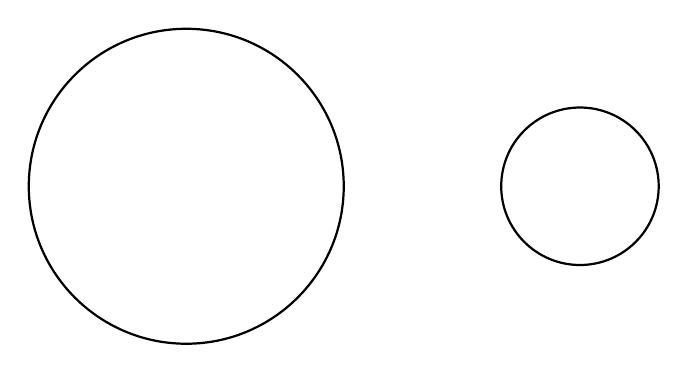
\begin{tikzpicture}[scale=1,cap=round,>=latex]
    \draw[thick] (0cm,0cm) circle(2cm);
    \draw[thick] (5cm,0cm) circle(1cm);
\end{tikzpicture}
\caption{Two circles.}
\end{figure}


But from a topological point of view, the circles are ``the same.''
Each is just a circle.

How are they ``the same?''
Well, the specifics of \emph{topological equivalence} vary from problem to problem.
(We want to have the freedom to work with the notion that makes sense in a given situation.)
One thing that all notions of topological equivalence have in common is the idea of ``continuous deformation.''
The circles above are topologically equivalent because we can imagine slowly deforming the large circle into the small one by shrinking it, and at every point along the way our figure is still ``essentially a circle.''
We do not have to break the figure and reglue the ends.
We can just ``continuously deform'' the one shape into the other.

Of course, there are lots of shapes which can be continuously deformed into a circle.

\begin{figure}[h]
\centering
%\begin{tikzpicture}[scale=1]
%    \draw[very thick] (0,0) circle[x radius = 2 cm, y radius = 1 cm];
%\end{tikzpicture}
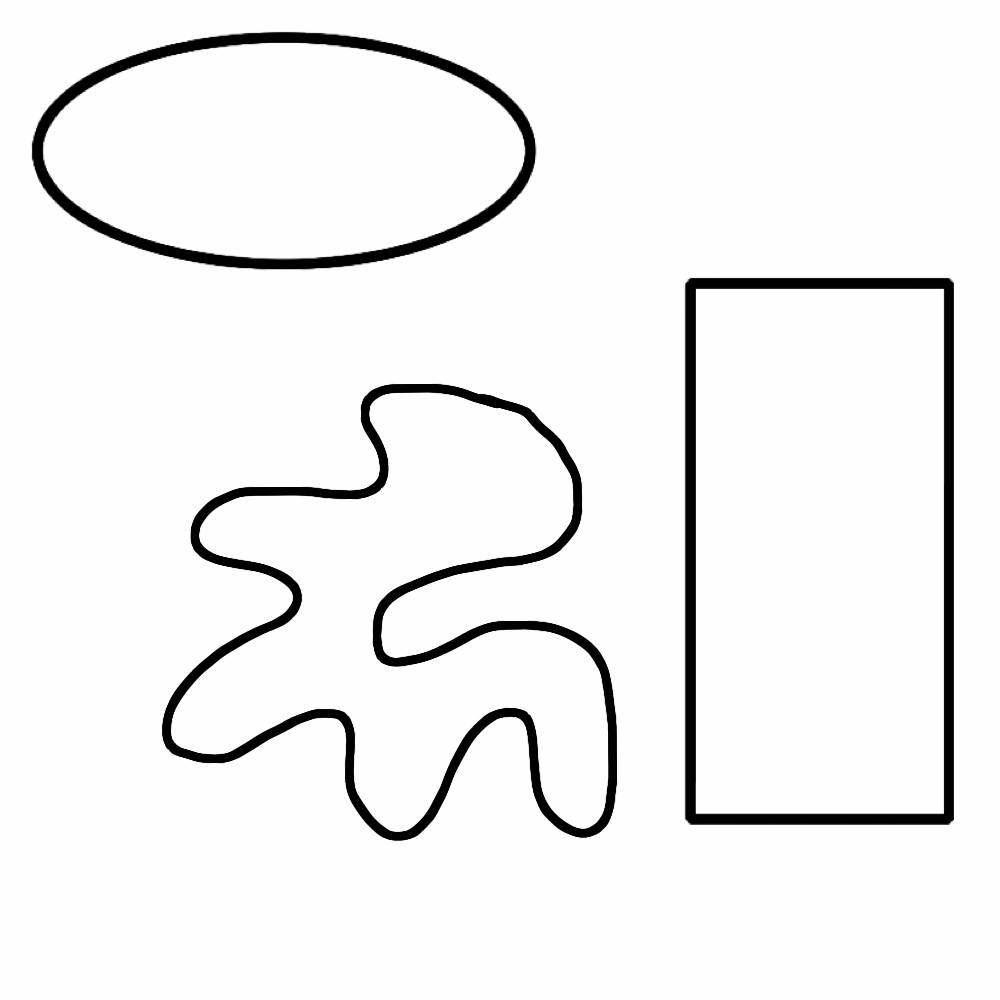
\includegraphics[height=3in]{rgp04pics/topcircle.png}
\caption{Three examples of  topological circles.}
\end{figure}

However, this figure eight in the plane is different!
\begin{figure}[h]
\centering
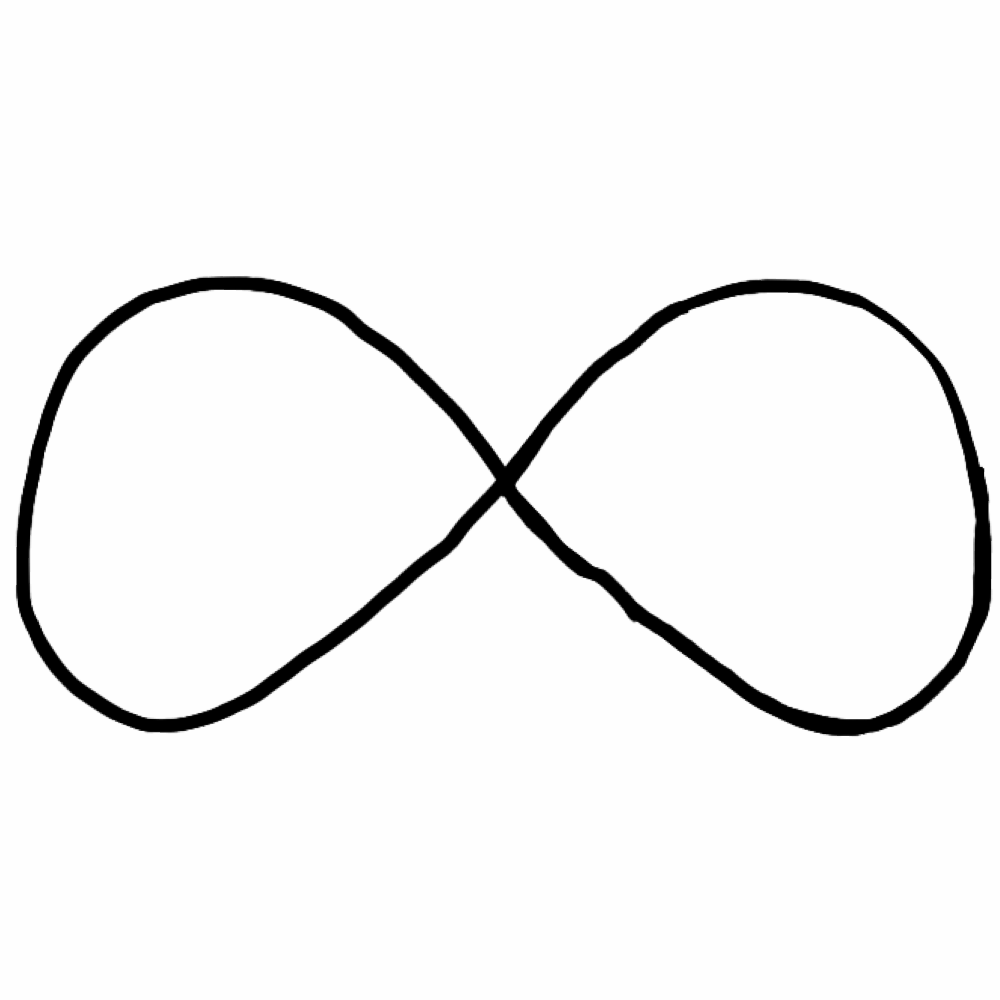
\includegraphics[height=2in]{rgp04pics/fig8.png}
\caption{Not a circle. Not even up to a continuous deformation.}
\end{figure}

There is a point where the curve crosses itself.
At that point, the shape looks more like an $+$ than a \textbar, and those shapes are distinguishable without measuring lengths or angles.


\subsection*{Topology and Picture Hanging Puzzles}

Where is the topology in the set of picture hanging puzzles?
Consider the two attempted solutions below.

\begin{figure}[h]
    \centering
    \begin{subfigure}[b]{0.4\textwidth}
        \centering
        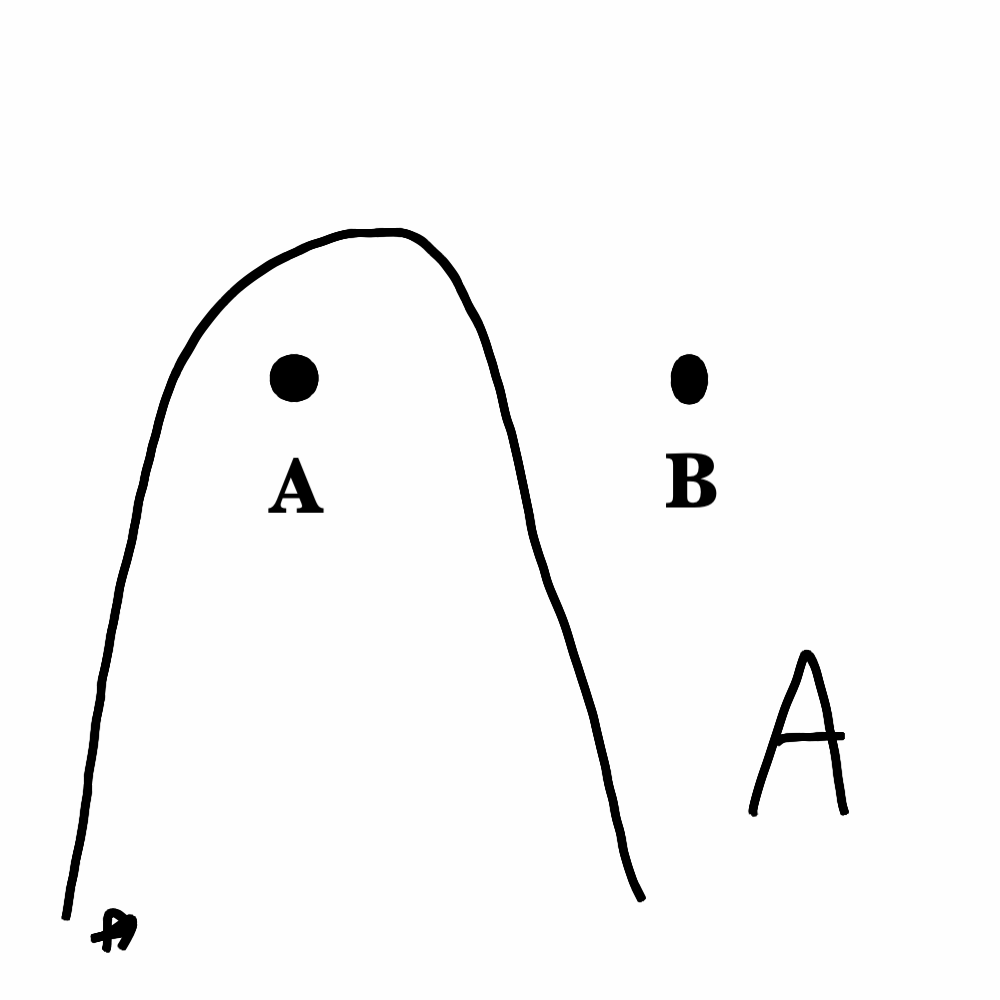
\includegraphics[width=\textwidth]{rgp04pics/A.png}
     \end{subfigure}
     \qquad
     \begin{subfigure}[b]{0.4\textwidth}
         \centering
         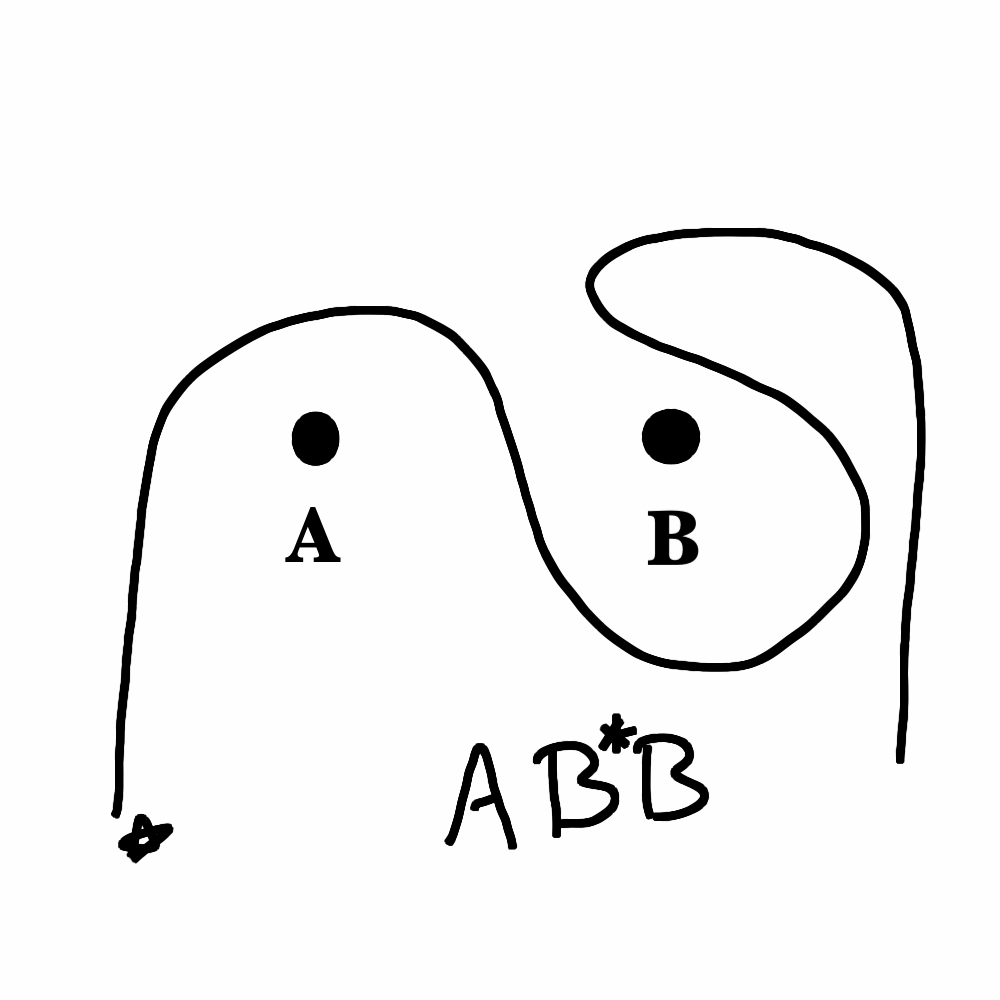
\includegraphics[width=\textwidth]{rgp04pics/ABsB.png}
     \end{subfigure}
\caption{Two topologically equivalent wire wrappings.}
\end{figure}

When you pull the wire down at the ends (by hanging the picture), you see that the loop $B^*B$ over nail B pulls out, and we get left with just $A$.
That ``pulling taut'' realizes a continuous deformation between the two situations.
These two arrangements are ``topologically equivalent,'' and that is the type of equality that is relevant to the question at hand.

Note that the following \emph{geometric} considerations are not important to us when solving picture hanging puzzles.
\begin{compactenum}
\item the distance between the nails;
\item the actual positions of the nails (If we move the nails a little bit, nothing important changes.); and
\item the thickness of the wire.
\end{compactenum}

\begin{task}
In your own words, describe what topology is and how it differs from geometry.
It might help to write this out in a paragraph.
It might help to tell a friend.
It would be very helpful to try out your explanation on a classmate and then discuss the similarities and differences between your descriptions.
\end{task}

\subsection*{Where else might topology be relevant?}

How do belt loops on a pair of pants make a belt more effective?
Topology!
The belt and the loops are \emph{linked}.
So the pants cannot fall down unless the belt goes too.

Now, keeping the belt up is a \emph{geometry} problem.
The length of the belt should be reasonably matched to the perimeter of some cross-section of the wearer.
But you knew that.

\begin{challenge}
Think of one or two other examples of situtations where topological properties are the important ones.
\end{challenge}

%\begin{thebibliography}{9}
%\end{thebibliography}

\end{document}
%sagemathcloud={"zoom_width":100}